\documentclass{article}

\usepackage{graphicx}
\usepackage{tikz}
\usepackage{tikzsymbols}
\usetikzlibrary{calc,patterns,shapes.geometric}
\pagestyle{empty}
\usepackage[margin=0pt]{geometry}
\geometry{papersize={14in,12in}}

\def\centerarc[#1](#2)(#3:#4:#5){\draw[#1] ($(#2)+({#5*cos(#3)},{#5*sin(#3)})$) arc (#3:#4:#5);}

\begin{document}
	\begin{figure}
		\centering
		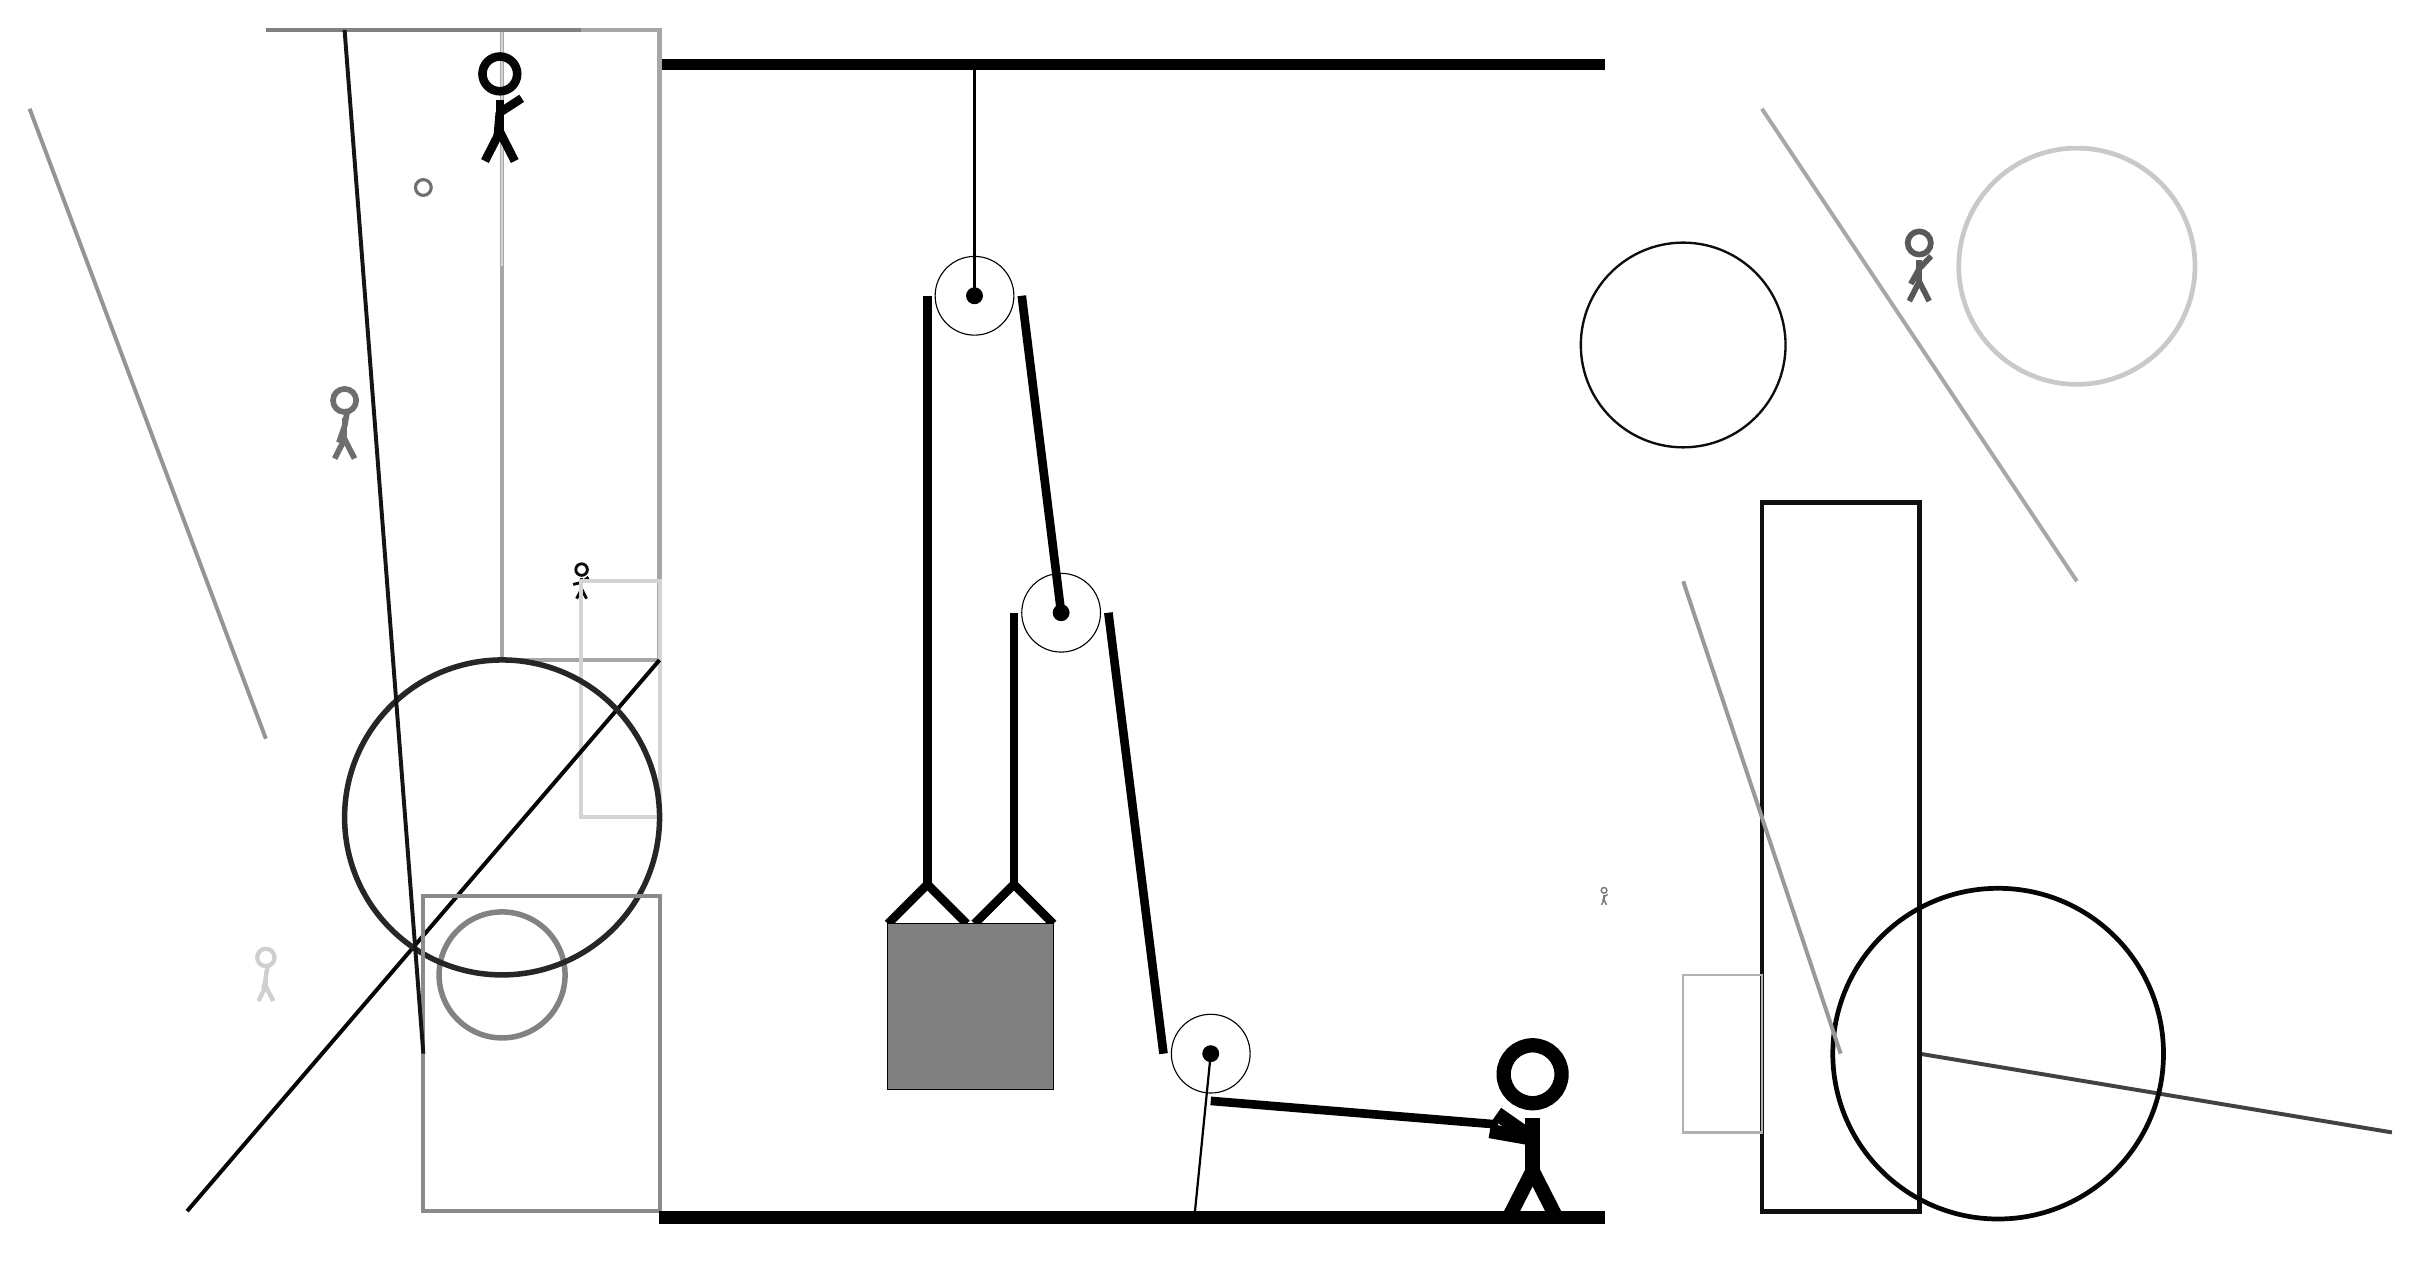
\begin{tikzpicture}
			%%%%% START %%%%%
			
			\draw[fill=black] (-2, 11.5) rectangle (10, 11.625);
			
			\draw (2, 8.625) circle (0.5);
			\draw[fill=black] (2, 8.625) circle (0.1);
			\draw[thick] (2, 8.625) -- (2, 11.5);
			
			\draw (3.1, 4.6) circle (0.5);
			\draw[fill=black] (3.1, 4.6) circle (0.1);
			
			\draw[line width=0.5mm, color=black!34](12, 11) -- (16, 5);
			
			\draw [line width=0.7mm, color=black!49](-4, 0) circle (0.8);
			\draw[line width=0.5mm, color=black!74](14, -1) -- (20, -2);
			\draw[line width=0.6mm, color=black!94] (12, -3) rectangle (14, 6);
			\draw[line width=0.6mm, color=black!35] (-4, 4) rectangle (-2, 12);
			\node[line width=0.3mm, color=black!96] at (-3, 5) {\Strichmaxerl[2][13][37]};
			\draw[line width=0.3mm, color=black!30] (11, 0) rectangle (12, -2);
			
			\node[line width=0.3mm, color=black!19] at (-7, 0) {\Strichmaxerl[3][79][81]};
			\draw [line width=0.4mm, color=black!56](-5, 10) circle (0.1);
			
			\draw[line width=0.3mm, color=black!16] (-4, 12) rectangle (-4, 9);
			\draw [line width=0.3mm, color=black!95](11, 8) circle (1.3);
			\draw [line width=0.6mm, color=black!98](15, -1) circle (2.1);
			\draw[line width=0.5mm, color=black!17] (-2, 5) rectangle (-3, 2);
			\node[line width=0.4mm, color=black!57] at (-6, 7) {\Strichmaxerl[4][71][80]};
			\node[line width=0.6mm, color=black!52] at (10, 1) {\Strichmaxerl[1][73][33]};
			\draw[line width=0.5mm, color=black!40](11, 5) -- (13, -1);
			
			\node[line width=0.2mm, color=black!98] at (-4, 11) {\Strichmaxerl[6][85][33]};
			\draw[line width=0.5mm, color=black!98](-2, 4) -- (-8, -3);
			\draw[line width=0.5mm, color=black!42](-7, 3) -- (-10, 11);
			\draw [line width=0.7mm, color=black!85](-4, 2) circle (2.0);
			\draw [line width=0.6mm, color=black!21](16, 9) circle (1.5);
			
			\node[line width=0.2mm, color=black!65] at (14, 9) {\Strichmaxerl[4][61][47]};
			\draw[line width=0.5mm, color=black!46] (-2, -3) rectangle (-5, 1);
			\draw[line width=0.5mm, color=black!50](-7, 12) -- (-3, 12);
			\draw[line width=0.5mm, color=black!92](-5, -1) -- (-6, 12);
			
			
			\draw (5, -1) circle (0.5);
			\draw[fill=black] (5, -1) circle (0.1);
			\draw[thick] (5, -1) -- (4.8, -3);
			
			\draw[line width = 1.1mm]  (0.9, 0.65) -- (1.4, 1.15) -- (1.9, 0.65);
			\draw[line width = 1.1mm]  (2.0, 0.65) -- (2.5, 1.15) -- (3.0, 0.65);
			\draw[fill=black!50] (0.9, 0.65) rectangle (3.0, -1.45);
			
			\draw[line width = 1.1mm] (1.4, 8.625) -- (1.4, 1.15);
			\centerarc[line width = 1.1mm](2, 8.625)(0:180:0.6);
			\draw[line width = 1.1mm] (2.6, 8.625) -- (3.1, 4.6);
			\draw[line width = 1.1mm] (2.5, 4.6) -- (2.5, 1.15);
			\centerarc[line width = 1.1mm](3.1, 4.6)(0:180:0.6);
			\draw[line width = 1.1mm] (3.7, 4.6) -- (4.4, -1);
			\centerarc[line width = 1.1mm](5, -1)(180:270:0.6);
			\draw[line width = 1.1mm] (5, -1.6) -- (8.65, -1.9);
			
			\node at (9, -2) {\Strichmaxerl[10][-35][170]};
			
			\draw[fill=black] (-2, -3) rectangle (10, -3.15);
			
			%%%%% END %%%%%
		\end{tikzpicture}
	\end{figure}	
\end{document}